\documentclass[12pt,twoside]{reedthesis}
\usepackage[hyphens]{url}
\usepackage{amsmath}
\usepackage{amssymb}
\usepackage{amsthm}
\usepackage{booktabs}
\usepackage{caption}
\usepackage{enumitem} 
    \setlist[itemize]{itemsep=1pt}
\usepackage{graphicx}
\usepackage{latexsym} 
\usepackage{longtable}
\usepackage{rotating}
\usepackage{setspace} 
\usepackage{xcolor} 
\usepackage{graphicx}
\graphicspath{ {./images/} }
\usepackage{ulem} % strikethrough
%\usepackage{natbib}
%\usepackage[style=reading,backend=bibtex8]{biblatex} \addbibresource{bibliography.bib}
\setlength{\parskip}{0pt}
\newcommand{\red}[1]{\textcolor{red}{#1}}
\newcommand{\green}[1]{\textcolor{olive}{#1}}
\newcommand{\todo}{\red{TODO}}
\newcommand{\comment}[2]{\textbf{#1} \textcolor{blue}{#2}}
\newcommand{\addressed}[2]{{#1}}

\title{A Survey of Superoptimizers}
\author{Elijah Wheelock}
\date{May 2024}
\division{Mathematics and Natural Sciences}
\advisor{Greg Anderson}
\department{Computer Science}
\begin{document}
\maketitle
\frontmatter % roman number these pages
\pagestyle{empty} % remove page numbers from the frontmatter
\chapter*{Acknowledgements}
I'd like to thank Greg, Tobey, Jennifer, Arthur, Norman, Susan, and Elise.
\tableofcontents

\chapter*{Abstract}
    % \red{TODO:} FIXME: punch up first couple sentences, end with ``this is a survey".

    Superoptimization is a family of compilation techniques which seek to improve the characteristics of computer programs by computational means.
    In this paper, we will survey a variety of methods from the literature which have been used for superoptimization.
    We systematized these techniques according to their approach to the problem of generating new programs.

\mainmatter % arabic number these pages
\pagestyle{fancyplain} % turn page numbering back on
\chapter*{Introduction}
    \addcontentsline{toc}{chapter}{Introduction} % includ intro in ToC
    \chaptermark{Introduction}
    \markboth{Introduction}{Introduction} % fix headers; % don't number intro as 1 so that chapter one is 1
    \singlespacing % \onehalfspacing % \doublespacing
    
    %   \red{TODO:} Reiterate abstract in introduction
    %\\ \red{TODO:} keep reorganizing
    
    One way to look at the history of life is as a long climb towards greater intelligence.
    One way to look at intelligence is as a tool for the performance of computations.
    It's natural when performing a computation to wish that it should work faster.
    Therefore the task of computational optimization is fundamental to life.
    
    Removing our tongues from our cheeks, we still are left with the desire to improve our programs. 
    Traditional approaches in this field generally do so by means of an optimizing compiler, which rewrite programs using a large number of essentially find-and-replace transformation rules.
    There is currently a wide variety of other approaches to this problem in the literature, ranging from tools for the education of programmers, to formal machine reasoning software, to multi-million-dollar so-called ``AI" systems.
    In an attempt to keep things relatively concrete, for the purposes of this thesis, we have chosen to focus mainly on one type of program: sequences of assembly/machine code, and one way of improving them: unguided search.
    
    Our formal problem statement is the following: given a specification program in a formal language $L$, produce an equivalent program in $L$ which scores better on a given metric.
    Most often the metric will be code size or performance (speed), but others are possible.
    
    Before we dive into superoptimization properly, it seems good to briefly discuss the traditional approach\footnotemark.
    A traditional compiler has (roughly) three main stages, commonly called the frontend, the middle-end, and the backend.
    Each part rewrites the program in such a way as to make the next part possible.
    A compiler, like a superoptimizer, takes as input a specification program in a formal language $L$, but rather than returning an equivalent program in $L$, it produces a program in a new language $L'$ (often but not always binary machine code), in accordance with the formal syntactic and semantic specifications of $L$ and $L'$.
    The frontend parses the input code, to ensure that it is a syntactically meaningful program in the language of the compiler, and to transform the unstructured text of the code into a richer data structure called an abstract syntax tree, which is much easier to reason about programmatically.
    The middle-end performs some high-level transformations on the syntax tree, such as dead code elimination and constant propagation.
    This type of reasoning is very much akin to some of the dataflow reasoning done by some of the superoptimizers we will soon see in Chapter 1. 
    At some point during the processing done by the middle-end, it transforms the abstract syntax tree again, into another language that's somewhere between a syntax tree and a simplified assembly language, called an \textit{intermediate representation} (IR).
    This IR is the input to the final part of the compiler, the backend.
    The backend performs the final processing steps necessary to produce the final assembly code, such as register selection and instruction scheduling.
    
    \footnotetext{
    For a more complete exploration of this topic, see one of the many high-quality textbooks on the subject, e.g. \cite{cooper2022engineering}.
    }
    
    \green{
    Like a compiler, a superoptimizer works in three main stages: synthesis, pruning (optional), and verification.
    The synthesis and pruning stages are cooperative -- the synthesizer produces a family of candidate programs, and the pruner decides which (if any) of them are worth investigating.
    If the pruner accepts a candidate, or if there's no pruner, it's then passed to the verifier. 
    If it passes the verifier, then depending on the system, it may be passed to the user for further review, or considered correct and used as-is.
    }
    
    \green{
    Another way to look at things is that superoptimization recharacterizes the problem of program improvement as a search problem, rather than an equational reasoning problem.
    This is seen as distinct from ``traditional" optimization (perhaps more properly called meliorization), which seeks to improve programs by application of a large number of rewrite rules.
    This is desirable because it allows the use of a wide variety of techniques from the literature on unguided search problems.
    More broadly, superoptimization may be seen as an application of the techniques of program synthesis to the domain of concretely-realized (assembly code/IR) programs.
    In practice, there is an infinite number of potential programs which compute the desired result, many of which are not intuitively obvious.
    Therefore it is desirable to have special techniques for synthesizing, pruning, and verifying such candidate programs. 
    }

\chapter{Symbolic Search}
    %   \red{TODO:} Chapter intro: what is symbolic search?
    %\\ \red{TODO:} talk about guaranteed progress, timeouts, etc.
    \green{
    One straightforward possible strategy when faced with a superoptimization problem is to attempt to ``solve" it symbolically. 
    Such approaches have the advantage that they will eventually find a solution, if one exists.
    Since they make guaranteed progress, in theory the length of synthesized program is limited only by the user's patience and available computing power.
    }
    
    \section{Enumeration}
        \subsection{Superoptimizer -- A Look at the Smallest Program}
            \green{
            Perhaps the simplest possible approach, pioneered by Henry Massalin in \cite{massalin1987superoptimizer}, is simple enumeration. 
            The word ``superoptimizer" dates from this paper.
            The technique is to line up all possible programs "alphabetically" in order of length, testing each in turn by the selected verification strategy. 
            }
                
            The synthesis stage in this system is the simplest imaginable: simply write down all assembly programs in alphabetical order.
            The advantage of this approach is that if a result is found, it will be the smallest possible code that can compute the desired result.
            In the loop-free case, this is likely also the fastest result -- running fewer instructions is generally preferable.
            However, on many architectures, the latency for instructions varies -- for example, division may be more expensive than multiplication, which may be more expensive than addition \cite{fog2022instructiontables}.
            The disadvantage is that the search space blows up exponentially with the length of function sought, making it intractable for all but the smallest code segments.
                
            The pruning stage is also relatively simple.
            There are some obviously-spurious code sequences if what is sought is the shortest possible correct code, e.g. ``move X,Y; move Y,X".
            Code containing such sequences may be rejected early, before the more-expensive verification stage.
                
            Massalin gives two distinct approaches to verification, driven by resource limitations.
            The reliable, but slow and expensive way, is to logically test the bitwise equivalency of the candidate program to the desired program, using what Massalin calls a ``boolean program verifier".
            As we'll see soon, this approach has become much more practical in the years since then, due to improvements both in hardware and SMT solvers. 
                
            This system, although relatively simple, and harshly limited by the available computation hardware of its era, achieves some qualitatively interesting results -- for example, Massalin uses it to search for efficient instruction sequences to divide by constants, but fails to find any.
            Since the superoptimizer performs an exhaustive search, this constitutes a proof that there are no such sequences. (Presumably these constants were not powers of two, division by which can be accomplished by a right shift.)

        \subsection{Automatic Generation of Peephole Superoptimizers}
            One clever way to reduce the expense and inconvenience associated with running a superoptimizer to improve your code is to precompute it
            -- that is, to cache the results of superoptimizing common code segments, and use these results as part of the peephole stage of an ordinary optimizer.
            Such is the strategy adopted by Bansal and Aiken \cite{bansal2006peephole}.
            
            This system works by harvesting code segments from a large corpus of existing programs, with certain restrictions, and superoptimizing them. 
            In contrast to Massalin's superoptimizer, it uses a runtime-estimate based cost function, as opposed to length-based.
            Rather than simply counting up the number of instructions, it adds up their cycle times, as referenced from the Intel technical manual.
            This gives a better approximation of the true runtime of the code segment.
            
            The selection of code segments is somewhat involved.
            One problem that might occur with superoptimizing a code segment is that it might disturb invariants relied on by other parts of the program.
            When the code segment is selected manually, this is not a problem.
            But for automatic selection, the system has to be confident that the segments won't be jumped into from elsewhere.
            For example, if the superoptimizer were to work on a code segment containing the start of a loop, but not the end, it would become difficult where the target of the jump at the end of the loop should be, especially if instructions are deleted or reordered.
            Another problem that could occur is that the update of the loop index variable could be lost or moved, in which case the semantics of the overall program are most likely made nonsense.
            
            It also uses a different pruning strategy.
            Before testing an instruction sequence, it is first canonicalized by renaming the registers it uses in a consistent way.
            If the canonicalized form has already been checked, then the sequence may be safely pruned.
            
            The verification strategy is similar to Massalin's boolean verifier, but using a SAT solver.
            This approach had become much more practicable in the intervening time between these publications due to algorithmic and hardware advances -- see e.g. \cite{silva1996grasp}.
            
            Bansal and Aiken's system achieves quite impressive results -- a speedup by a factor of between 1.7 and 10, (mean ~4.9) in compute-intensive programs, with a 1-5\% speedup in more general programs, all compared to code already nominally optimized by the compiler.

    \section{SMT}
        Satisfiability modulo theories (SMT) is family of extensions to the classic problem in computer science of boolean formula satisfiability (known as SAT).
        The SAT problem is, given a formula of boolean logic composed of 
                the boolean operators 'and', 'or', and 'not';
                parentheses;
                and an arbitrary number of variables each of which may take the value of either 'true' or 'false',
            to determine whether there exists a \textit{satisfying assignment} of values to variables such that the overall formula can be reduced to 'true'.
        SAT was proven to be NP-complete in \cite{cook1971sat}, and so is widely considered to be intractable in the general case.
        Furthermore, depending on the theories used, SMT problems may be fully undecidable.
        However, in practice many of the problems that naturally arise in various fields, including in program synthesis, are able to be solved in reasonable time by specially constructed solver programs, for example Z3 \cite{demoura2008z3}.
        Z3 is commonly used in program synthesis, and adds theories of variable equality, arithmetic, fixed-size bit-vectors, arrays, and quantifiers.

        \green{
        A reasonably complete explanations of the workings of a SMT solver would be beyond the scope of this work.
        The interested reader may wish to read \cite{demoura2008z3} and \cite{dpll1962theorem}.
        }

        \subsection{Denali: A Goal-directed Superoptimizer}
            Another early work on superoptimization, by Joshi et al. \cite{joshi2002denali} uses an automated theorem prover to simultaneously synthesize and verify new programs.
            It takes a program in a custom low-level language, expresses it in a symbolic form as a graph of all equivalent ways of computing its output expressions
                \addressed{called the E-graph}{I would be inclined to have a separate description of E-graphs, but it depends on the structure of the section},
                and \green{uses that to generate input for a SAT solver.}
            
            \green{
            Generating the E-graph is a fairly complicated process, since matching terms in a graph is not trivial.
            Denali uses a special graph matching algorithm by some of the same authors, described in \cite{detlefs2005simplify}.
            It uses a set of mathematical axioms as augmentation rules to generate a graph where each node is an equivalence class of expressions for each term of the input program. It does this until it reaches a fixed point, i.e. no more matches can be made and thus each equivalence class is complete.
            For example, if one term in the specification is $x * 2$, it would use the fact that multiplication by one is equivalent to left-shifting by one to augment that term to the equivalence class $\{x * 2, x \ll 1\}$.
            }
            
            \footnotetext{That is to say that, like a compiler, it has a set of rules by which it re-writes expressions. For each rule, it searches the document for that rule's the left-hand-side, and replaces it with the right-hand-side, and repeats until no more substitutions are possible.}
                
            The connections between the E-graph nodes are then translated into clauses for the use of the SAT solver.
            \green{
            Denali formulates the conjecture that ``no program of the target architecture computes the values of the goal terms within $K$ cycles" as an input to a satisfiability solver.
            }
            In order to logically express the number of cycles required for the whole program, it has to express the time by which every intermediate step will be completed.
            To do this, Denali uses an additional set of constraints on the times of launching, completion, and availability, which may be roughly summarized by the following slogans:
            \begin{itemize}
                \item A computation is completed after its latency has elapsed since its launch time.
                \item A computation can't be launched until its arguments are available.
                \item A value is available at all times at or after its completion time.
                \item Only one operation may be launched per cycle (The paper gives some remarks on extending to multiprocessing systems, but does not explain in detail).
            \end{itemize}
            
            The results section in this paper is not extensive, but they report that Denali was able to meet or exceed the performance of an aggressively-optimizing C compiler on certain problems.

        \subsection{Unbounded Superoptimization}
            A more modern take on a similar approach to Denali is the work by Jangda and Yorsh in ``Unbounded Superoptimization" \cite{jangda2017unbounded}.
            Rather than matching E-graphs, which in the intervening years had been integrated into SMT solvers, it directly encodes the target program as a logical formula.
            It does this by encoding the input program, treating it as the first candidate output, and ``squeezing" it by imposing lower and lower cost bounds on the solver.
            This ``top-down" approach has the advantage that if the superoptimizer is halted early, it can still return a correct output, unlike many superoptimizers which work ``bottom-up" and thus start without any candidate programs.

            \green{
            There are three types of constraints in the model:
                the semantics of the input code $p$;
                the semantics of an arbitrary bounded-length instruction sequence in the target architecture $a$;
                and an equivalence constraint $o$ that enforces the property that the output program have the same observable behavior as the input.
            Then the input to the solver at each step is of the form 
            \[
                \forall x, x', y, y' ~:~ \hat{p} \wedge \hat{a} \wedge \hat{o}
            \]
                where $\hat{p}$ is a symbolic representation of $p$;
                $x$ and $x'$ are the input and output of $p$ respectively;
                $y$ and $y'$ are the input and output of the candidate program;
                $\hat{o}$ is the observable equivalence constraint;
                and $\hat{a}$ is the symbolic representation of the semantics of $a$, which can be paraphrased as 
            \[
                \hat{a} := \forall j < n \;:\; \bigwedge_{i \in I} \left((j^\text{th} \text{ instruction is } i) \Rightarrow [(\text{state at time } j + 1) = \tau_i(\text{state at time }j)]\right)
            \]
            where $n$ is the length of the candidate to generate, $I$ is the set of possible instructions in $a$, and $\tau_i$ is the semantics of instruction $i$.
            The ``squeezing'' step is accomplished by adding an additional constraint that $n < n'$, where $n'$ is the length of the current best candidate.
            }
            
            Jangda and Yorsh tested their technique on a set of problems from Hacker's Delight \cite{warren2013hackers}.
            They successfully generated optimal code for 17 of 25 problems, and failed for 8.
            Comparing the output of their technique to the outputs of \texttt{gcc -O3}\footnotemark, they found that for 3 of the problems the code generated by their tool was about 20\% faster than (and algorithmically distinct from) the output of \texttt{gcc -O3}; on the other 14 problems the performance was identical to that of \texttt{gcc -O3}.
            
            \footnotetext{
            \texttt{gcc} is the Gnu Compiler Collection (originally, the Gnu C Compiler; it now supports many languages), one of the highest-quality optimizing compilers for C programs.
            It's common for compilers to offer (at least) four different optimization levels, from {-O0} to {-O3}, where {-O0} is more-or-less a direct translation of the source program, and {-O3} is the highest level of compiler aggression that remains standard-compliant.
            (It's common practice in industry to use {-O2} as standard, because writing perfectly standard-compliant C code is not trivial.)
            }

    \section{CEGIS}
        Counter-example guided inductive synthesis (CEGIS) is a program synthesis technique introduced by Solar-Lezama et al. in \cite{solar-lezama2006sketch}.
        Like some of the other techniques we've seen so far, it takes a specification program and computes an output which satisfies the specification (if possible).
        However, rather than rewriting the specification to be more efficient, like a superoptimizer, it takes an additional input, an incomplete program called a ``sketch", and computes appropriate program fragments to fill one or more ``holes" left in the sketch by the user.
        Its output is then the completed sketch, transformed into a fully-functioning implementation of the specification, or an error, if such an implementation is impossible.
        
        \green{
        CEGIS works by using two cooperating SMT solver instances, one to generate new possible program completions, and another to generate counterexample inputs that possibly rule out those completions.
        Formally, the CEGIS system from the original paper\footnotemark attempts to solve the following boolean formula, where $P$ is the specification program and $S$ is the sketch:
        \[
            \exists c \in \{0,1\}^k,\; \forall x \in \{0,1\}^m \text{ such that } P(x) = S(x,c)
        \]
        First, it generates a random input $x$ to the sketch, and uses the first solver to find a candidate pregram completion $c$ such that $S(x,c) = P(x)$. 
        If it can't find such a completion, then the specification is considered incorrect, and an error is returned.
        If it does find an appropriate $c$, it then uses the second solver to attempt to verify that the equation $S(x,c) = P(x)$ holds for \textit{all} $x$.
        If it is, then the sketch is completed; otherwise, the counterexample provided by the second solver is added to the set of inputs $I$ considered by the first solver, so that in future iterations it attempts to find $c$ such that the formula
        \[
                \bigwedge_{x\in I} S(x, c) = P(x)
        \]
        holds.
        }

        \footnotetext{
        The original paper covered only the synthesis of constants; later papers extended the idea to larger programs.
        The interested reader may wish to look at \cite{gulwani2011loopfree}.
        }
        
        \subsection{Souper: A Synthesizing Superoptimizer}
            Souper \cite{sasnauskas2017souper} is an engineering project to create a superoptimizer working on LLVM intermediate representation (IR).
            This is desirable because LLVM is used as the ``middle end" for a large number of compiler projects, and therefore Souper can be used for a wide variety of languages and target architectures.
            It has three main components:
                an extractor, to produce Souper IR from LLVM IR,
                a synthesizer using counterexample-guided interactive synthesis,
                and a verifier using an SMT solver.
            
            Souper uses a custom IR analogous to a purely-functional subset of LLVM IR without control flow\footnotemark, represented for computational purposes as a directed acyclic dataflow graph.
            It is also limited to integer instructions; it has no model for floating-point, memory, or vector operations.
            The operands of programs in this IR are considered only as bitvectors (parameterized by width) or tuples of bitvectors.
            
            \footnotetext{Some information about control flow external to the code segment under consideration is preserved, but control flow operations within a code segment are forbidden.}
            
            \green{
            To ensure that synthesized programs are low-cost, Souper wraps its CEGIS step in a loop: first it attempts to synthesize a zero-instruction program (only using a constant or an input), then a one-instruction program, then a two-instruction program, and so on.
            Thus its cost function is simply the code size, or number of instructions.
            }
            
            \green{
            The authors spend some effort discussing some problems which might make Souper produce incorrect output.
            The most obvious possibility, which is of course a potential problem for any computer system, is a bug in Souper's implementation.
            However, they observed miscompilations arising from other problems as well, including a bug in the solver library they were using.
            Perhaps the most interesting, however, was Souper's exploitation of undefined behavior\footnotemark. 
            Souper asserts to the SMT solver that no undefined behavior may occur in either the specification or the generated program; therefore if a program accidentally depends on undefined behavior, Souper is even more likely to find and exploit it than a standard compiler, and the behavior of Souper's output may therefore be surprising.
            }
            
            \footnotetext{
            \green{
                Undefined behavior is a concept in certain programming languages, which attempt to specify the \textit{observable behavior} of the code generated by the compiler from compliant programs; however, if a program is considered non-compliant, the behavior of the code emitted by the compiler is considered completely unspecified.
                For example, signed integer overflow is considered undefined behavior by the C standard.
                This property of some specifications has been increasingly exploited by compiler writers, particularly in the C/C++ language community, to improve the performance of their compilers on certain benchmarks by making strong assumptions that code which may potentially exhibit undefined behavior will never encounter a situation in which it does so.
                This allows, for example, removing checks for signed integer overflow, because checking whether undefined behavior has occurred is by definition undefined.
            }
            }

        \subsection{Dataflow-Based Pruning for Speeding up Superoptimization}
            Mukherjee et al. \cite{mukherjee2020dataflow} enhance Souper with an additional family of pruning strategies based on dataflow reasoning. 
            Pruning spurious candidates as early as possible is obviously highly desirable, because every hole for a constant represents a potentially-costly invocation of the MST solver; a hole for a partial program is even worse, as it represents a possibly-infinite family of related candidates.
            This paper uses both \textit{forward} and \textit{backward} dataflow analysis techniques to prove candidate expressions incorrect before they are fully substantiated (while they still contain ``holes", constants or sub-expressions which have yet to be synthesized).
            Mukherjee et al. define forward techniques as those which work by drawing a chain of reasoning from properties of the specification program's output into properties which must hold for a correct candidate program.
            By contrast, backward techniques draw inferences from the program's inputs into the candidate.
            
            The forward techniques are known/bivalent bits and integer ranges.
            The backward techniques are required bits/don't-care bits and forced bits.
            
            The known-bits analysis works by proving that certain bits of the output of the candidate program are necessarily incompatible with the specification.
                For a simple example, if the specification ends by setting the rightmost bit of the output to 1, then any candidate which ends with a left shift can be immediately dismissed.
            The integer ranges analysis works by proving that there is some output of the specification that is outside the range of the candidate.
                For example, if we know that for the specification $f(x) = -1$ for some $x$, we can prune the candidate $g(x) = abs(x)$.
            
            The required-bits analysis works by proving that certain bits of the input to the specification are \textit{required}, i.e. that changing its value (with other bits constant) necessarily changes the output.
                If such an input is not used in a candidate program (is a don't-care bit), then that program can be safely pruned.
                    For example, if the specification is $x + y$, but the candidate is $x + C$ where $C$ is constant, the candidate may be pruned.
            The forced-bits analysis is in a way analogous to the known-bits analysis, working in the opposite direction.
                It works by finding conflicts in candidates with symbolic (not-yet-synthesized) constants.
                Intuitively, it can be thought of as finding inconsistencies in a system of equations based on comparing the candidate to the specification.
                For example, suppose the specification is $f(x) = x^2 + 1$, and the candidate is $g(x) = x + C$. In that case, $f(3) = 10$, and $f(1) = 2$. Then we need $C$ such that $f(3) = g(3) = 10 = 3 + C$, and $f(1) = g(1) = 2 = 1 + C$, so we must have $1 = C = 7$. This is unsatisfiable, so we can dismiss $g$ without attempting to learn anything more about it.
            
            Results: Mukherjee et al. tested the performance of Souper on 269,113 C/C++ programs from SPEC CPU 2017\footnote{https://www.spec.org/cpu2017/}, with and without the addition of their dataflow pruning techniques.
            The compiled outputs from LLVM served as the specifications for Souper.
            They considered a synthesis attempt a success only when it found a candidate with lower cost than the specification;
            they declared it a failure if it took too much time (300 seconds) or memory (4GB).
            They found that their pruning made Souper's synthesis 2.32x faster, and increased the number of successful syntheses finished before timeout by 8\%.
            Their pruning procedure took less than 3\% of the overall runtime of the synthesis attempts in which it was used.
            They found that pruning made synthesis faster for 87\% of problems; it was slower mainly for very large problems with hundreds of instructions.

        %Present CEGIS first, then decide if this is still in
        % \subsection{From Relational Verification to SIMD Loop Synthesis}
        % \cite{barthe2013simdloopsynth}

\chapter{Stochastic Search}
    Heretofore we have limited ourselves to superoptimizers which operate in a deterministic regime.
    However, there is another way to think of the problem: as an unguided search in a high-dimensional, irregular search space.
    While this way of thinking loses some desirable properties from more deterministic approaches, such as guaranteed progress or canonical ``solutions" for small problems, it also unlocks a variety of techniques for use in superoptimization, which may scale better\footnotemark\, than deterministic techniques.
    
    \footnotetext{In this context, ``scaling better" means that it becomes expensive more slowly, relative to input size. Remember that the space of possible programs grows exponentially with program length, so any optimizer which attempts to explore all of it will take a very long time for even relatively short programs!}

    \section{Markov Chain Monte Carlo Sampling}
    \subsection{Stochastic Superoptimization}
        Markov chain monte carlo (MCMC) sampling is a technique used to sample from complex possibility spaces, first used for superoptimization by Schkufza et al. in \cite{schkufza2013stoke}.
        Essentially, the strategy works by drawing candidate rewrites from a distribution with favorable properties (in this case, a bias toward low cost). \green{The desired distribution of candidate programs is given by the following:
        \[
            p(\mathcal{R;T}) = \frac{1}{Z} \mathrm{exp}\left(-\beta \cdot c(\mathcal{R;T})\right)
        \]
        where $p(\mathcal{R;T})$ is the probability of generating candidate rewrite $\mathcal{R}$ given target specification $\mathcal{T}$; $Z$ is a normalization constant so that sum of probabilities of all candidates adds up to 1; $\beta$ is a constant, and $c$ is the cost function. 
        Essentially, this distribution enforces the property that a more costly candidate is much less likely than a less costly one: a candidate with cost $n$ has probability proportional to $1/e^n$.
        }

        \green{
        Since it's difficult to draw from this distribution directly, the Metropolis-Hastings algorithm \cite{metropolis1953montecarlo} \cite{hastings1970mcmc} allows sampling from it indirectly by using a chain of rewrites.
        The algorithm maintains a current best candidate, and draws rewrites from a given pool.
        }
        A rewrite which scores better than the current candidate is always accepted; a worse one is accepted with probability proportional to $1/e^{(c'/c)}$, where $c$ is the cost of the old candidate and $c'$ is the cost of the new one. 
        \green{
        There are four rewrites in the pool used by \textsc{Stoke}: 
        \begin{itemize}
            \item Opcode: a random instruction is selected from the candidate and replaced by a random other instruction which take the same number and type of operands.
            \item Operand: a random instruction is selected from the candidate and one of its operands is replaced by a random one of the same type.
            \item Swap: two instructions from the candidate are swapped.
            \item Instruction: a random instruction is selected from the candidate and replaced by a random other instruction, or by a no-op
        \end{itemize}
        }
        
        Correctness is estimated by the hamming distance (bitwise difference: the number of corresponding bits that differ between the two strings, plus insertions, if needed) between the outputs of the candidate and those of the specification on the set of test cases.
        The test cases are generated based on annotations provided by the user; by default, they are uniformly random bitstrings.
        Cost is estimated by the sum of the (average) latencies of the instructions in the candidate.
        
        There are two phases to the search performed by \textsc{Stoke}:
            what they call synthesis, in which initially random programs are permuted to search for programs equivalent to the specification in disconnected parts of the search space,
            and optimization, in which correct programs are permuted in search of better performance.
        The top 20\% of candidates are then formally verified and tested for performance, and the best candidate is returned.
        
        Schkufza et al. test \textsc{Stoke} against 25 problems from Hacker's Delight \cite{warren2013hackers}, and 3 additional problems. 
        Beginning with the output of \texttt{llvm -O0}, it produced output which generally matched and in a few cases significantly exceeded that of \texttt{gcc -O3}.
        For 7 of 28 problems, it discovered programs which were algorithmically distinct from the input specification.
        For 3 of the problems, the synthesis step timed out, meaning that it was unable to derive an equivalent program \textit{de novo}; however, the optimization step was still able to discover a rewrite with good performance.

    \subsection{Conditionally Correct Superoptimization}
        One problem with the kind of bitwise verification accomplished by SMT solvers is that in some sense it's actually too exact.
        This has the disadvantages both of added expense for verifying more than necessary, and in rejecting correct but inexactly equivalent candidate optimizations.
        There are multiple reasons that successful optimizations might not be bitwise equivalent to the specification
            -- for example, the differences might only appear in a region of input space which is forbidden for some reason,
                e.g. if the difference only occurs for negative numbers, but we know that the input is the square of an integer
               (this is not a kind of example discussed in this paper, but it's an easily-explained example of the kind of reasoning involved).
        While there are a number of existing efforts to produce relaxation conditions from annotations given by the programmer to a traditional compiler, another possibility is to attempt to have the compiler generate them itself for review by the programmer.
        Such is the project of Sharma et al. in \cite{sharma2015conditionally}.
        
        This paper expands on \textsc{Stoke} with the intention of proving correctness more rigorously than the test-case based approach it originally used.
        It does this by augmenting it with a new verification algorithm, which they call \textsc{Cove} (described below).
        They name the version of \textsc{Stoke} thus augmented \textsc{cStoke}.
        \textsc{cStoke} works using a formal verification system for x86 assembly created by the same authors \cite{sharma2013ddec} (modulo certain pointer aliasing changes) to generate verification conditions for the candidate program produced by \textsc{Stoke}, which are then fed into \textsc{Cove} to produce a set of preconditions that make the target and candidate equivalent.
        These preconditions are then presented to the programmer, and if accepted, the candidate program is considered correct.
        
        The aliasing changes mentioned above constitute a relaxation of the formal verification process -- it turns out that reasoning about aliasing\footnotemark is a relatively expensive part of the verifier, and that it is the grounds for rejection for a large number of candidates.
        Therefore, rather than considering every possible case of pointer aliasing, only those which are relevant in the traces for the given test cases are considered.
        This does not affect the overall correctness of \textsc{Cove}, since the derived non-aliasing assumptions are included (explicitly or implicitly) in the final set of preconditions presented to the user.
        
        \footnotetext{Two pointers are said to be \textit{aliased} if the data they point to overlap.}
        
        The workings of \textsc{Cove} are as follows:
        The preconditions are generated from the verification conditions via abstract interpretation\footnotemark by conjoining abstractions of the test inputs on which the target and candidate are equivalent in progressively more-restrictive abstract domains.
        The domains used in \textsc{Cove} are bitvector alignment to 1, 2, 4, 8, 16, 32, and 64 bytes, bit-vector equalities, and bit-vector intervals (interpreted as intervals of unsigned integers).
        
        \footnotetext{
        Abstract interpretation is a means of over-approximating the behavior of programs.
        For example, we might abstract the integers in a program into the domain of sign, i.e. positive, negative, or zero.
        If we're multiplying our integers, this abstraction would still allow us to prove things about the final output;
        on the other hand, if we're adding them, then we'd have less information (for example, a positive times a negative is a negative, but a positive plus a negative is indeterminate).
        Thus different abstract domains are useful for reasoning about different questions.
        }
        
        % Greg: the abstraction function lifts a set of concrete values to the abstract domain--if you think of the abstract domain as some \emph{structured} set of inputs, then the abstract function enforces that structure while preserving overapproximation. The concretization function is the opposite--it ``forgets'' the structure of the abstract domain.
        
        Sharma et al. tested the performance of code generated by \textsc{cStoke} against code generated by \texttt{gcc -O3} and \texttt{icc -O3}\footnotemark on a wide variety of benchmarks, including common compiler benchmarks and some preexisting application programs.
        In the interest of fairness, they provided the compilers with annotations of the preconditions generated by \textsc{Cove}, insofar as that was possible.
        They found that \textsc{cStoke} always matched or exceeded \texttt{gcc}, and almost always matched or exceeded \texttt{icc}.
        Furthermore, on some programs, the code generated by \textsc{cStoke} was up to five times faster than code generated by \texttt{gcc}, and up to six times faster than that generated by \texttt{icc}.
        
        \footnotetext{\texttt{icc} is the Intel C Compiler.}

    \subsection{Scaling up Superoptimization}
        Perhaps it's a natural question, when comparing the strengths and weaknesses of various superoptimization techniques, to ask, ``why not use them all together, and let the strengths of each cover the weaknesses of the others?"
        Phothilimthana et al. attempt precisely this in \cite{phothilimthana2016scaling}.
        They also spend considerable effort comparing and contrasting results achieved by various techniques.
        
        This paper uses multiple techniques for synthesis in a ``cooperative superoptimizer".
        \textsc{Lens}, a new enumerative superoptimization algorithm,
        a sliding-window strategy to decompose programs too large to superoptimize directly,
        and a synthesizer combining communicating symbolic, stochastic, and enumerative search programs.
        
        \green{
        \textsc{Lens} is an enumerative algorithm.
        It builds up candidate programs from both forwards and backwards directions, by working from the input/output pairs from a set of test cases.
        When it finds a program bridging between the input and output, it attempts to verify it using an SMT solver.
            If the solver verifies it, then it's a correct instantiation of the specification, and so it's returned.
            If the solver finds a counterexample input, that input and its corresponding output are added to the set of test cases from which new candidates will be generated.
        }

        \green{
        When generating candidate programs it uses a reduced bitwidth.
        In their experiments, this reduced 32-bit programs to 4 bits.
        This simplifies the implementation of the reverse synthesis step; instead of needing a reverse emulator they can get away with a lookup table for $2^4$ input/output pairs for each instruction.
        This also mitigates the combinatorial explosion from backwards synthesis -- an instruction in the forward direction is one-to-one, but in the backward direction this is not necessarily the case. 
        For a simple two-bit example, suppose our input $11$ is the left-hand side in the equation $11 \wedge 01 = 01$.
        In the forward direction this is fully known.
        But since we lose information in the forward direction, in the reverse direction we have multiple possible completions for the left-hand side -- in particular, it's impossible to know if the input should have been $01$ or $11$.
        Therefore \textsc{Lens} must track both possibilities if it's to guarantee finding a solution (if one exists).
        This explosion of possibilities is much, much worse in 32 bits than in 2 or 4!
        }

        \green{
        \textsc{Lens} accomplishes the bitwidth reduction by simply replacing each constant $c$ with $c \mod 2^\text{bitwidth}$, unless $c$ is a shift operand, in which case it does some special processing meant to preserve the semantics of shift operations in the newly-reduced domain.
        This replacement is memorized, so that it can be undone when it's time to verify a candidate.
        }
        
        The sliding window strategy is fairly simple; it randomly picks a window of the program to superoptimize, attempts to improve it, and repeats until no position of the window yields an improvement to the program.
        There is one additional detail that bears mentioning: 
            this window decomposition allows the verification step to use the context of the surrounding program when checking equivalence;
            rather than checking equivalence of the candidate with the target, it can check the equivalence of the sequence prefix-candidate-suffix with the sequence prefix-target-suffix.
        This allows a few additional optimizations.
        
        The strategies used in the ``cooperative superoptimizer" are
        \begin{itemize}
            \item \textsc{Lens} on the whole program,
            \item \textsc{Lens} with window decomposition,
            \item an SMT solver on the whole program,
            \item an SMT solver with window decomposition,
            \item \textsc{Stoke} starting from a random program, and
            \item \textsc{Stoke} starting from the specification program.
        \end{itemize}
        The communication between synthesizers takes the form of a shared best solution, $p_{best}$.
        The whole-program \textsc{Lens} and SMT synthesizers don't use $p_{best}$. The others restart their synthesis, using $p_{best}$ as the new starting point instead of the target.
        
        \green{
        Phothilimthana et al. tested the components of their system in a variety of ways. We have summarized the most interesting results in the following list:
        \begin{itemize}
            \item They tested \textsc{Stoke} vs the whole-program SMT solver vs whole-program \textsc{Lens}; they found that \textsc{Lens} was faster and solved more of their benchmark programs than their implementations of either of the others.
            \item They tested multiple versions of \textsc{Lens} with and without a number of strategies; they found that their pruning strategies improved search speed by 11 times.
            \item They tested the cost of programs produced by \textsc{Lens} with and without the sliding window decomposition, and found that it did not make a consistent improvement to cost.
            \item They tested their whole cooperative system vs a system running one whole-program \textsc{Lens} instance and a large number of sliding-window \textsc{Lens} instances, providing equal computational resources to both systems; they found that the cooperative superoptimizer was 33\% faster and solved\footnote{matched best-known solutions for} more of their benchmark problems.
            \item They tested the speed of the code generated by their system against that generated by \texttt{gcc -O3} and found that their code met or exceeded \texttt{gcc}'s on all benchmark programs.
        \end{itemize}
        }
        
        \begin{center}
            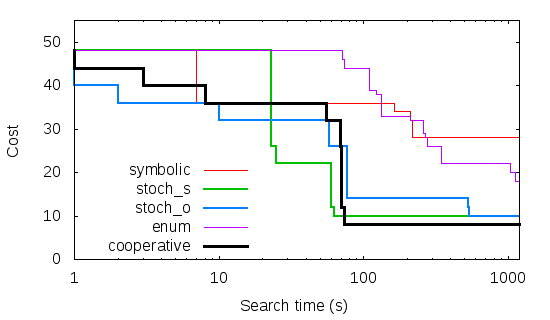
\includegraphics[scale=0.5]{scaling}
            \captionof{figure}{ \green{ An example comparison of the process of optimizing a program by five different superoptimizers: 'symbolic' is an SMT solver; 'stoch\_s' and 'stoch\_o' are \textsc{Stoke} starting from a random program and from the specification respectively; 'enum' is \textsc{Lens}; 'cooperative' is the whole system together.} }
        \end{center}

    % on backburner
    %\subsection{Sound Loop Superoptimization for Google Native Client}
    %\cite{churchill2017soundloop}

    \section{Reinforcement Learning}
        \green{
        Machine learning using neural networks is a field which has seen significant successes in recent years, so it's only natural that we should see attempts to use it for superoptimization. 
        }
        Reinforcement learning is a machine learning paradigm useful for cases when the structure of a problem is not straightforwardly numeric, but an objective function of the success/failure of an attempted output is available.
        This function is called the reward/loss function, depending on its sign. In such cases neural networks may be trained by gradient ascent on the reward function or gradient descent on the loss function.
        % REINFORCE: REward Increment = Non-negative Factor $\times$ Offset Reinforcement $\times$ Characteristic Eligibility
        % for RL focus on loss/reward fn
        
        Due to Sutton et al. in \cite{sutton1999policygradient}, the gradient may be calculated by the following expression:
        \[
            \frac{\partial \rho}{\partial \theta} = \sum_s d^\pi(s) \sum_a \frac{\partial \pi(s,a, \theta)}{\partial \theta}Q^\pi(S,a),
        \]
        where $\theta$ is the vector of policy parameters, $\rho(\pi)$ is the (long-term) expected reward from following policy $\pi$, $d^\pi$ is the (stationary) distribution of states expected under $\pi$, and $Q^\pi(s,a)$ is the long-term expected reward from following policy $\pi$ starting from a given state-action pair.
        
        This formulation \textit{requires} that $\pi$ be differentiable with respect to $\theta$, i.e. that $\frac{\partial \pi(s,a, \theta)}{\partial \theta}$ exists.
        The reason this formulation is convenient is that there is no term of the form $\frac{\partial d^\pi(s)}{\partial \theta}$, i.e. the effect of policy changes on the distribution of states is irrelevant.
        This allows the gradient to be conveniently estimated by sampling.

        %\subsection{Learning Performance-Improving Code Edits} \cite{}

        \subsection{Learning to Superoptimize Programs}
            % Augment \textsc{Stoke} by using reinforcement learning to improve the distribution of proposed mutations.
            % two different techniques: learning bias and multilayer perceptron
            One natural objection to the techniques used in \textsc{Stoke} is that in an optimal program, some instructions are more likely than others.
            Bunel et al. attempt to apply this insight in \cite{bunel2017learning}.
            They use reinforcement learning to train two different models of the desired policy:
                an unconditional bias for \textsc{Stoke}'s mutation algorithm,
                and a multi-layer perceptron\footnotemark,
                    which attempts to estimate the best mutations to make based on the instructions already present in the candidate under consideration.
            \footnotetext{A perceptron is a simple neural network which classifies its input into predetermined categories.}
            
            They train the systems using the expected cost of the output of the system, which can be paraphrased as the following loss function:
            \[
                \mathcal{L}(\theta) = \mathbb{E}_{\{\mathcal{R}\sim q_\theta}[r\{\mathcal{R}\}],
            \]
            where $q_\theta$ is the policy distribution, $r$ is the cost estimator for a rewrite, and $\{\mathcal{R}\}$ is a set of rewrites sampled from the policy distribution.
            
            Bunel et al. compare their biased version of \textsc{Stoke} with the original and with an unoptimized reference implementation.
            They find that the biased version significantly outperforms the original.
            On the Hacker's Delight problems, \textsc{Stoke} found programs with on average 53\% of the cost of the unoptimized implementation, while the biased version found programs with 32\% of the cost.
            On a set of random programs, \textsc{Stoke}'s average cost was 78\% of the unoptimized cost, while the biased version's average cost was 63.56%.
            The multi-layer perceptron achieved very slightly higher performance than the bias, improving on it by about 1\%.

        \subsection{Deep Symbolic Superoptimization Without Human Knowledge}
            Another reasonable desire when creating a superoptimization system is to manipulate programs directly via neural networks.
            Hui et al. attempt to do this in \cite{hui2020deep}. 
            The goal of this project is to rewrite expression trees to smaller equivalent forms. 
            It uses a three-stage system:
            \begin{itemize}
                \item an encoder network\footnotemark, which produces a vector for each subtree of the input
                \item a subtree selector, which tries to select promising subtrees to focus on
                \item a decoder/simplifier network, which tries to write an equivalent but smaller expression to the input.
            \end{itemize}
            
            \footnotetext{An encoder network maps its input, in this case a tree, to a vector; a decoder naturally does the reverse.}
            
            They train the system using the following reward function:
            \[
                R(\mathcal{T}_I,\mathcal{T}_O) =
                    \begin{cases}
                        \gamma^{\text{card}(\mathcal{T}_O)} & \text{ if } \mathcal{T}_I \equiv \mathcal{T}_O,
                    \\ -\beta\gamma^{\text{card}(\mathcal{T}_O)} & \text{ otherwise}
                    \end{cases}
            \] % explain equivalence relation
            where $\mathcal{T}_I$ is the input specification, $\mathcal{T}_O)$ is the candidate tree, $\gamma$ and $\beta$ are constants with $0 < \gamma < 1$, and $\text{card}(\mathcal{T})$ is the number of nodes in a tree.
            Effectively, this function prioritizes correct output, and between equivalent outputs, prefers shorter ones.
            They use an additional loss function when training the encoder which attempts to force equivalent expressions to have similar encodings, given by
            \[
                L = \frac{1}{|\mathbb{S}|} \sum_{\mathcal{T}_O \in \mathbb{S}} || \boldsymbol{h}(\mathcal{T}_O) - \boldsymbol{h}(\mathcal{T}_I) ||^2_2 \cdot (-1)^{\mathbb{I}[\mathcal{T}_O \not\equiv \mathcal{T}_I]}
            \]
            where $\mathbb{S}$ is a set of outputs generated via the decoder from the same input using beam search\footnotemark, $\boldsymbol{h}(\mathcal{T})$ is the embedding of $\mathcal{T}$ generated by the encoder, and $\mathbb{I}$ is the indicator function, which returns 1 when its argument expression is true, and 0 otherwise.
            
            \footnotetext{Beam search is a greedy search algorithm which attempts to pursue the most-promising candidates first. It discards less-promising candidates, thereby trading guaranteed completion for memory efficiency.}

        \subsection{Learning to Superoptimize Real-World Programs}
            Another attempt at a similar problem is made by Shypula et al. in \cite{shypula2022learning}.
            With this paper we return to the assembly superoptimization task which has been our focus through most of this document. 
            They use a transformer model\footnotemark in a supervised learning approach which attempts to learn input-output matching for assembly programs, with unoptimized binaries (\texttt{gcc -O0}) being used as the input examples, and optimized binaries (\texttt{gcc -O3}) being used as the outputs.
            
            \footnotetext{Transformers are a sequence-to-sequence machine learning model introduced in 2017 by Vaswani et al. in \cite{vaswani2017attention}, which translate ``words" of the input sequence into vectors so that they can be directly manipulated by a neural net; they are distinct from autoencoders in that they have an additional ``attention" mechanism, whereby words from a sliding context window are scored for importance before being processed by the main net.}
            
            The SILO algorithm essentially consists of replacing the outputs from the training set when a better one is found for a given input, then continuing training.
            
            The loss function can be paraphrased as 
            \[ L = P(F_o) \cdot (\text{cost}(F_o) + \lambda \cdot \text{correctness}(F_o) - b(F_I)), \]
            where $P$ is a term representing the probability of generating output function $F_o$, cost($F$) is the sum of the expected latencies for the instructions in $F_o$ (the same cost function as \textsc{Stoke}) plus the sum of the expected latencies of the instructions actually executed by $F_o$ on the test suite, correctness($F$) is 0 if $F$ is equivalent to $F_I$ and 1 otherwise, $\lambda$ is a tuneable penalty for incorrectness (they set it to 50000), and $b(F_I)$ is a baseline cost for the input function.
            
            They test the SILO system against REINFORCE alone, and find that SILO improves on \texttt{gcc -O3} on 8.9\% of their test set, as opposed to 0.9\% for REINFORCE.
            They found that REINFORCE consistently made improvements only on the same few problems from the test set, while SILO improved its performance with training.

\chapter{Conclusion}
    % \red{TODO:} future work?, comparison of techniques, 
    % conclusion:
        % briefly summarize intro, talk about different approaches again, advantages & disadvantages
        % more results-focused
        % if I've noticed open directions, point them out
    
    In conclusion,
        since the introduction of the term by Henry Massalin in \cite{massalin1987superoptimizer},
        a wide variety of techniques have been harnessed to the goal of superoptimization,
        which we have divided into two main categories by synthesis type:
            symbolic and stochastic,
        and five subcategories:
            enumerative, SMT, CEGIS, MCMC, and reinforcement learning.
    This is certainly not the only reasonable taxonomy for this problem.
    One list of possible taxonomies is the following:
        \begin{itemize}
            \item the techniques used for synthesis, as in this paper;
          % \item the techniques used for verification of generated programs;
            \item the goals (optimization criteria) of the superoptimization system;
            \item the problem domain;
            \item the capabilities/limitations of the system.
        \end{itemize}
    We'll discuss each of these alternatives briefly.
    
    As we've discussed now at some length, superoptimizers can be categorized by the approach they take to synthesis of superoptimized programs.
    This is the measure on which published systems vary most widely, and the selection of approach is perhaps the most salient question for the authors of new systems.
    These approaches vary widely in sophistication, complexity, and power.
    
    There are quite a few possible criteria by which to rank candidate programs.
    The most immediately salient is performance, and that is the one we have primarily focused on;
    in almost every application, faster programs are preferred to slower ones.
    However, performance is only one instance of another very reasonable goal, which is to reduce resource use.
    There are a number of resources whose conservation might be desired, for example:
    \begin{itemize}
        \item time and/or number of computers required for a computation, as we've discussed;
        \item memory usage;
        \item functional units on an FPGA;
        \item power or space on a hardware design;
        \item disk writes;
        \item or disk or network bandwidth.
    \end{itemize}
    To the best of our knowledge, most of these resources have not been the target of any published superoptimization system, mostly for good reasons;
    nevertheless, this may be an interesting direction for future work.
    A less-common criterion is to reduce the code size of generated programs.
    This might be desired for reasons such as:
    \begin{itemize}
        \item performance (using number of instructions executed as a crude measure of computation time, as we've seen);
        \item performance (improving performance directly by reducing instruction cache misses or instruction pipeline delays);
        \item the output code is meant to run on a resource-poor system such as a microcontroller;
        \item entertainment (``code golfing").
    \end{itemize}
    
    Another way to categorize superoptimizers is by the limits they set on their problem domain.
    For example, a common limitation is that the output code must be expressible in a loop-free way
        -- loops are a difficult problem for many approaches, not least because verifying equivalence of programs with arbitrary loop conditions is in general undecidable \cite{turing1937tm} \cite{sipser2012computation}, and because heuristic testing of loops may require unbounded time.
    
    Another common limitation in superoptimizers is that it's very difficult to produce an accurate cost estimation for memory access.
    Modern computer systems generally have many-layered information storage systems, with multiple layers of caching, batching, and indirection between them, making the estimation of latency for any particular memory access very difficult.
    For this reason, black-box measurement of performance (running the code on physical hardware) is the gold standard, but this is sometimes cost-prohibitive.
    For this reason many superoptimizers do not model programs which access memory in any way.
    
    Another limitation is that the overall difficulty of any search problem scales with the size of the search space, which in superoptimization scales exponentially with the length of the synthesized program.
    Therefore most superoptimization systems are strongly limited by available computation power, and performance reasons impose a maximum practical synthesized program size.
    This is particularly problematic when searching for constants; there may be dozens of possible operands for a register-to-register instruction, but an instruction with an embedded constant has $2^\text{bitwidth}$ possibilities.
    Depending on the synthesis technique, this may be more or less of an issue; 
    \textsc{Stoke} type synthesizers really struggle with constants, while CEGIS-types are designed to handle this issue.
    
    Another possible taxonomy is by problem domain.
    Many superoptimizers focus on assembly programs with integer operands, because there are powerful techniques for verifying such programs, but by no means all.
    There have also been interesting superoptimizers targeting 
    \begin{itemize}
        \item floating-point assembly programs, 
        \item compiler intermediate representation (IR) programs, 
        \item and high-level synthesis (HLS) languages for integrated circuit (IC) or field-programmable gate array (FPGA) development.
    \end{itemize}
    
    Overall, each of the techniques we've seen has its own strengths and weaknesses, and there is no overall ``best" strategy invented so far. 
    Enumerative superoptimizers have the benefit of simplicity at the cost of inefficiency;
    SMT-type superoptimizers get to take advantage of the advances made in theorem-proving and SAT-solving technology, which is still an area of active research;
    CEGIS-type superoptimizers build on SMT superoptimizers with a more advanced strategy for program synthesis;
    \textsc{Stoke}-type superoptimizers are better-equipped to work on longer programs;
    and RL-type superoptimizers get to take advantage of modern advances in machine learning models and parallel computing power.
    One possible direction for future research is the use of two or more of these techniques in a cooperative superoptimizer, distinct from the one used in \cite{phothilimthana2016scaling} by using its subunits in a hierarchical rather than parallel way. For example, a CEGIS-type optimizer might use its own synthesis strategy for holes that it expects to be small, and a \textsc{Stoke}-type strategy for holes that it expects to be large.

%\appendix
%\chapter{Appendix 1}

\backmatter
%\nocite{*} 
%\printbibliography
\bibliographystyle{alpha}
\bibliography{bibliography}
% To force capitalization in an article title or where all lowercase is generally used, bracket the capital letter in curly braces.
% optionally, an index would go here.

\end{document}
